\chapter{Hauptcharaktere}
\section{Soldat} \label{sec:mc-soldat}
\begin{itemize}
	\item männlich
	\item Alter:\\
	- 16 Jahre während Demo
	\item Aussehen:\\
	- dargestellt in Abb. \ref{fig:mc-soldat} \\
	- rötliche Haare, bis zu den Augenbrauen\\
	- Sommersprossen\\
	- sonnengebrannte Haut\\
	- strammer Typ
	\item Kleidung:\\
	- praktikabel\\
	- mit etwas Schutz
	\item Charakter:\\
	- bodenständig \\
	- optimistisch \\
	- charmant 
	\item Abstammung:\\
	- Vater: hochdekorierter Militär, nie Zuhause. War mal im Dorf stationiert -> dadurch mit Mutti zusammen gekommen\\
	- Mutter: stammt aus dem Dorf, liebevolle Beziehung\\
	- Geschwister: mind. 1 offen
	\item Hintergrund:\\
	- aufgewachsen im Kerndorf\\
	- hohes Interesse an den stationierten Soldaten, verbringt Freizeit auch gerne bei denen\\
	- eifert seinem Vater nach, will aus dem Dorf raus\\
	- eher wohlhabend
\end{itemize}

\begin{figure}
	\centering
	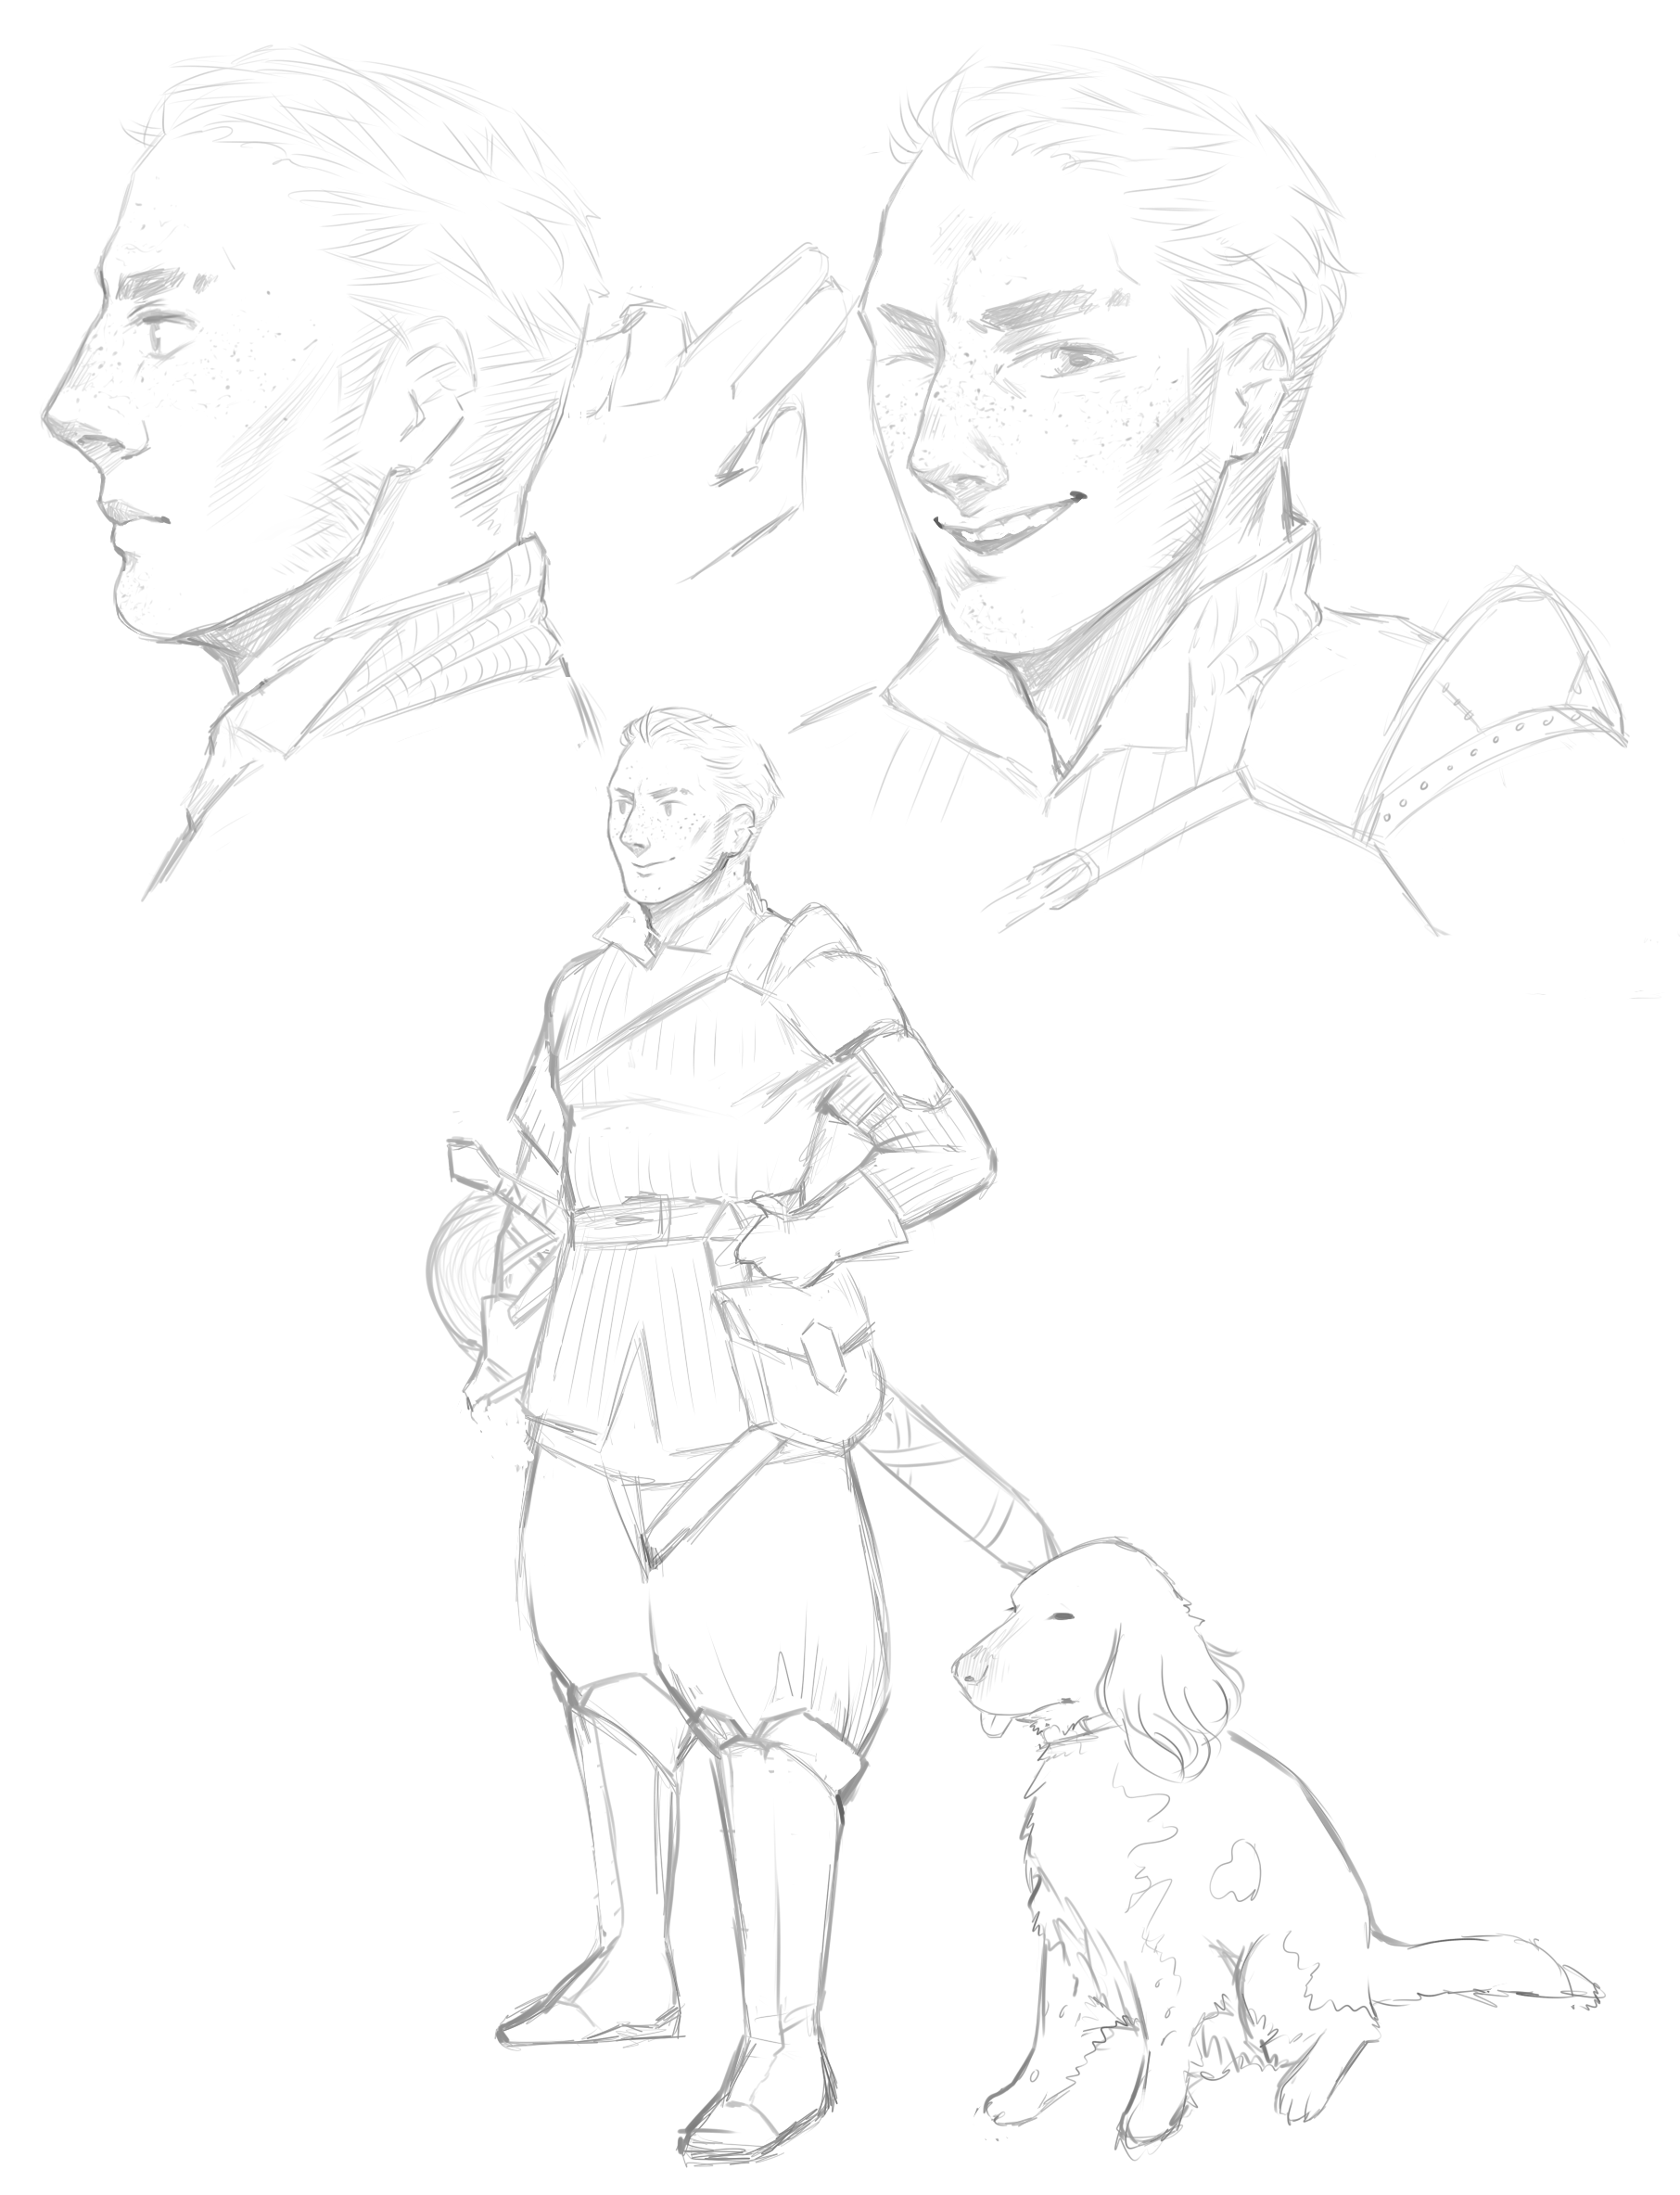
\includegraphics[width=0.75\textheight]{Abbildungen/Abenteuer/Hauptcharaktere/soldat.png}
	\caption[Konzeptart Soldat]{Konzeptart Soldat als 16-Jähriger während dem Hauptteil der Demo.}
	\label{fig:mc-soldat}
\end{figure}

\section{Diplomatin} \label{sec:mc-diplomatin}
\begin{itemize}
	\item weiblich
	\item Alter:\\
	- 17 zur Demo
	\item Aussehen:\\
	- wie dargestellt in Abb. \ref{fig:mc-diplomatin} \\
	- gut gepflegt \\
	- geschminkt
	\item Kleidung:\\
	- legt Wert auf Äußeres\\
	- lange Kleider
	\item Charakter:\\
	- "Mädchen"\\
	- ihr ist die Ehre der Familie sehr wichtig \\
	- legt viel Wert darauf, was andere von ihr halten \\
	- sehr offen gegenüber den schlechter beglückten
	\item Abstammung:\\
	- Mutter: die Geistliche im Amt, eingereist\\
	- Vater: deren Mann, Städter, musste mit seiner Frau mit. Während der Char ein Kind ist, ist er noch sehr unglücklich, später hat er sich mit einigen Männern angefreundet und sich mit der Situation zurechtgefunden. Arbeitet bei einem der innerdörflichen Berufe mit\\
	- Geschwister: mind. 3 offen
	\item Hintergrund:\\
	- absolut gläubig erzogen\\
	- eifert ihrer Mutter darin nach, eine hohe Position im Orden zu erlangen und diesem weiter zu helfen
\end{itemize}

\begin{figure}[h]
	\centering
	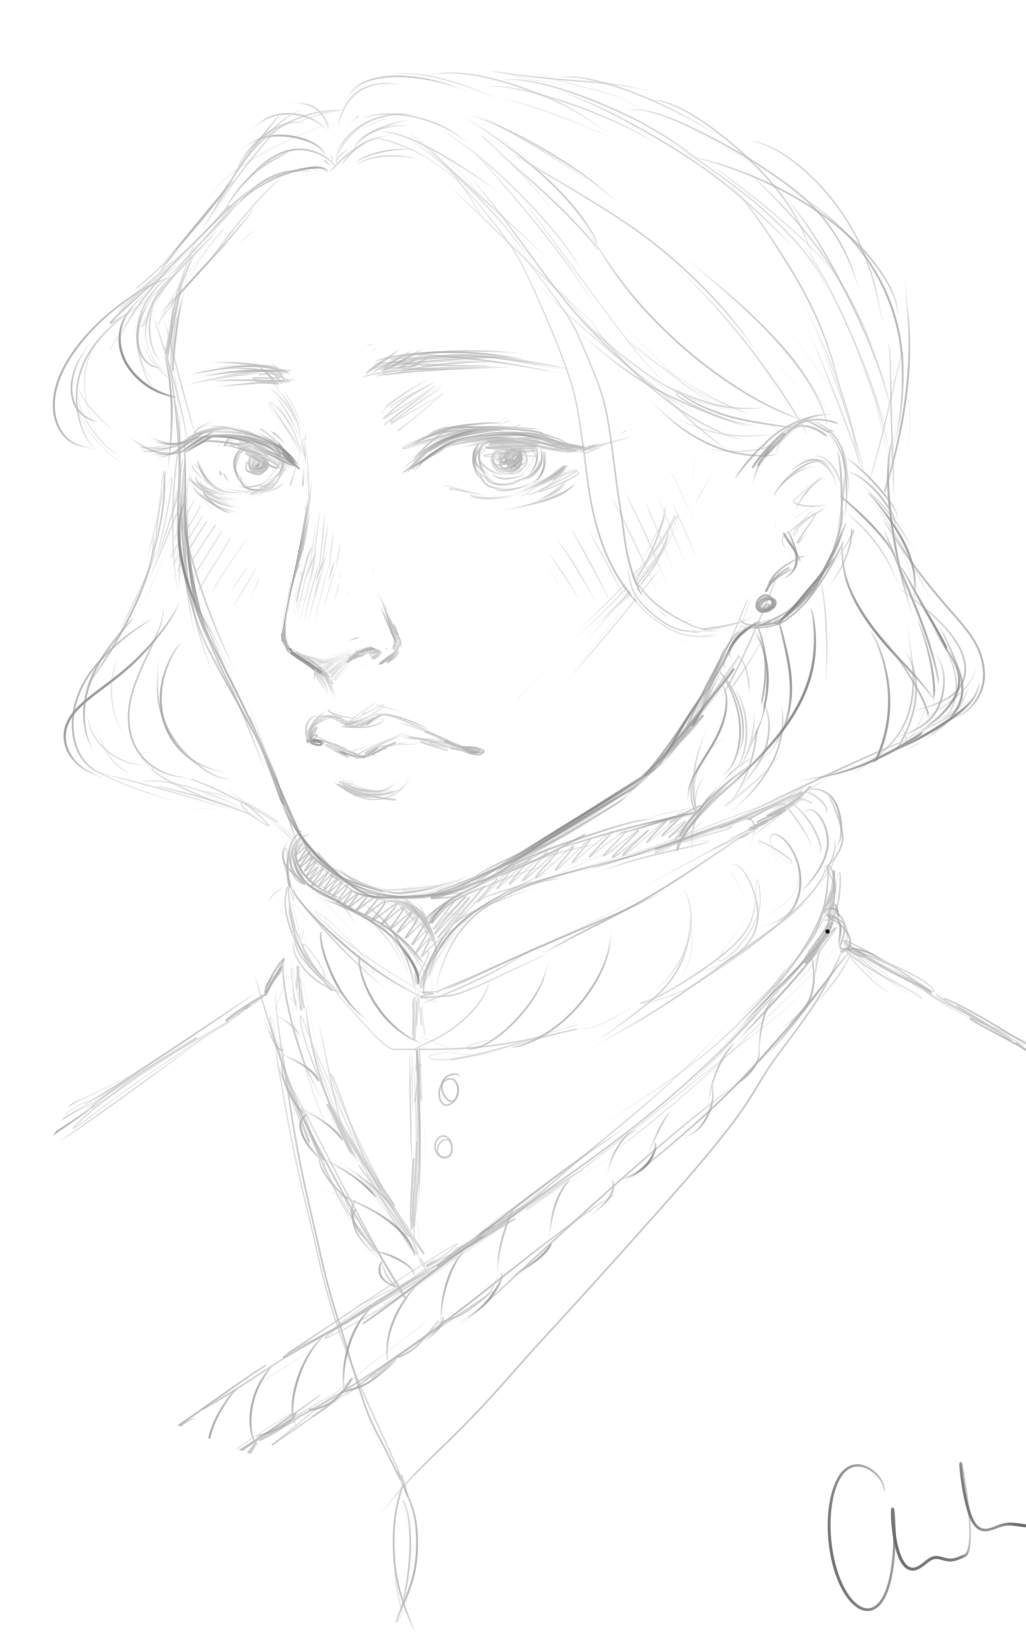
\includegraphics[width=0.325\textheight]{Abbildungen/Abenteuer/Hauptcharaktere/magierin}
	\caption[Konzeptart Diplomatin]{Konzeptart Diplomatin als 17-Jährige während dem Hauptteil der Demo.}
	\label{fig:mc-diplomatin}
\end{figure}


\section{Spionin} \label{sec:mc-spionin}
\begin{itemize}
	\item weiblich
	\item Alter:\\
	- 16 zur Demo
	\item Aussehen:\\
	- wie dargestellt in Abb. \ref{fig:mc-spionin}\\
	- Zopf bis Brust
	\item Kleidung:\\
	- praktisch\\
	- Hosen \\
	- Bogen, Dolch (zum Ausnehmen Wild) am Gürtel\\
	- Gugel?
	\item Charakter:\\
	- praktisch veranlagt\\
	- Wildfang \\
	- zynisch \\
	- schwarzer Humor
	\item Abstammung:\\
	- Vater: Jäger\\
	- Mutter: \\
	- Geschwister: einige offen
	\item Hintergrund:\\
	- arme und ungebildete Familie\\
	- aufgewachsen am Rand des Dorfes oder ggf. am Waldrand bei den 2-3 Jägerhütten
\end{itemize}

\begin{figure}
	\centering
	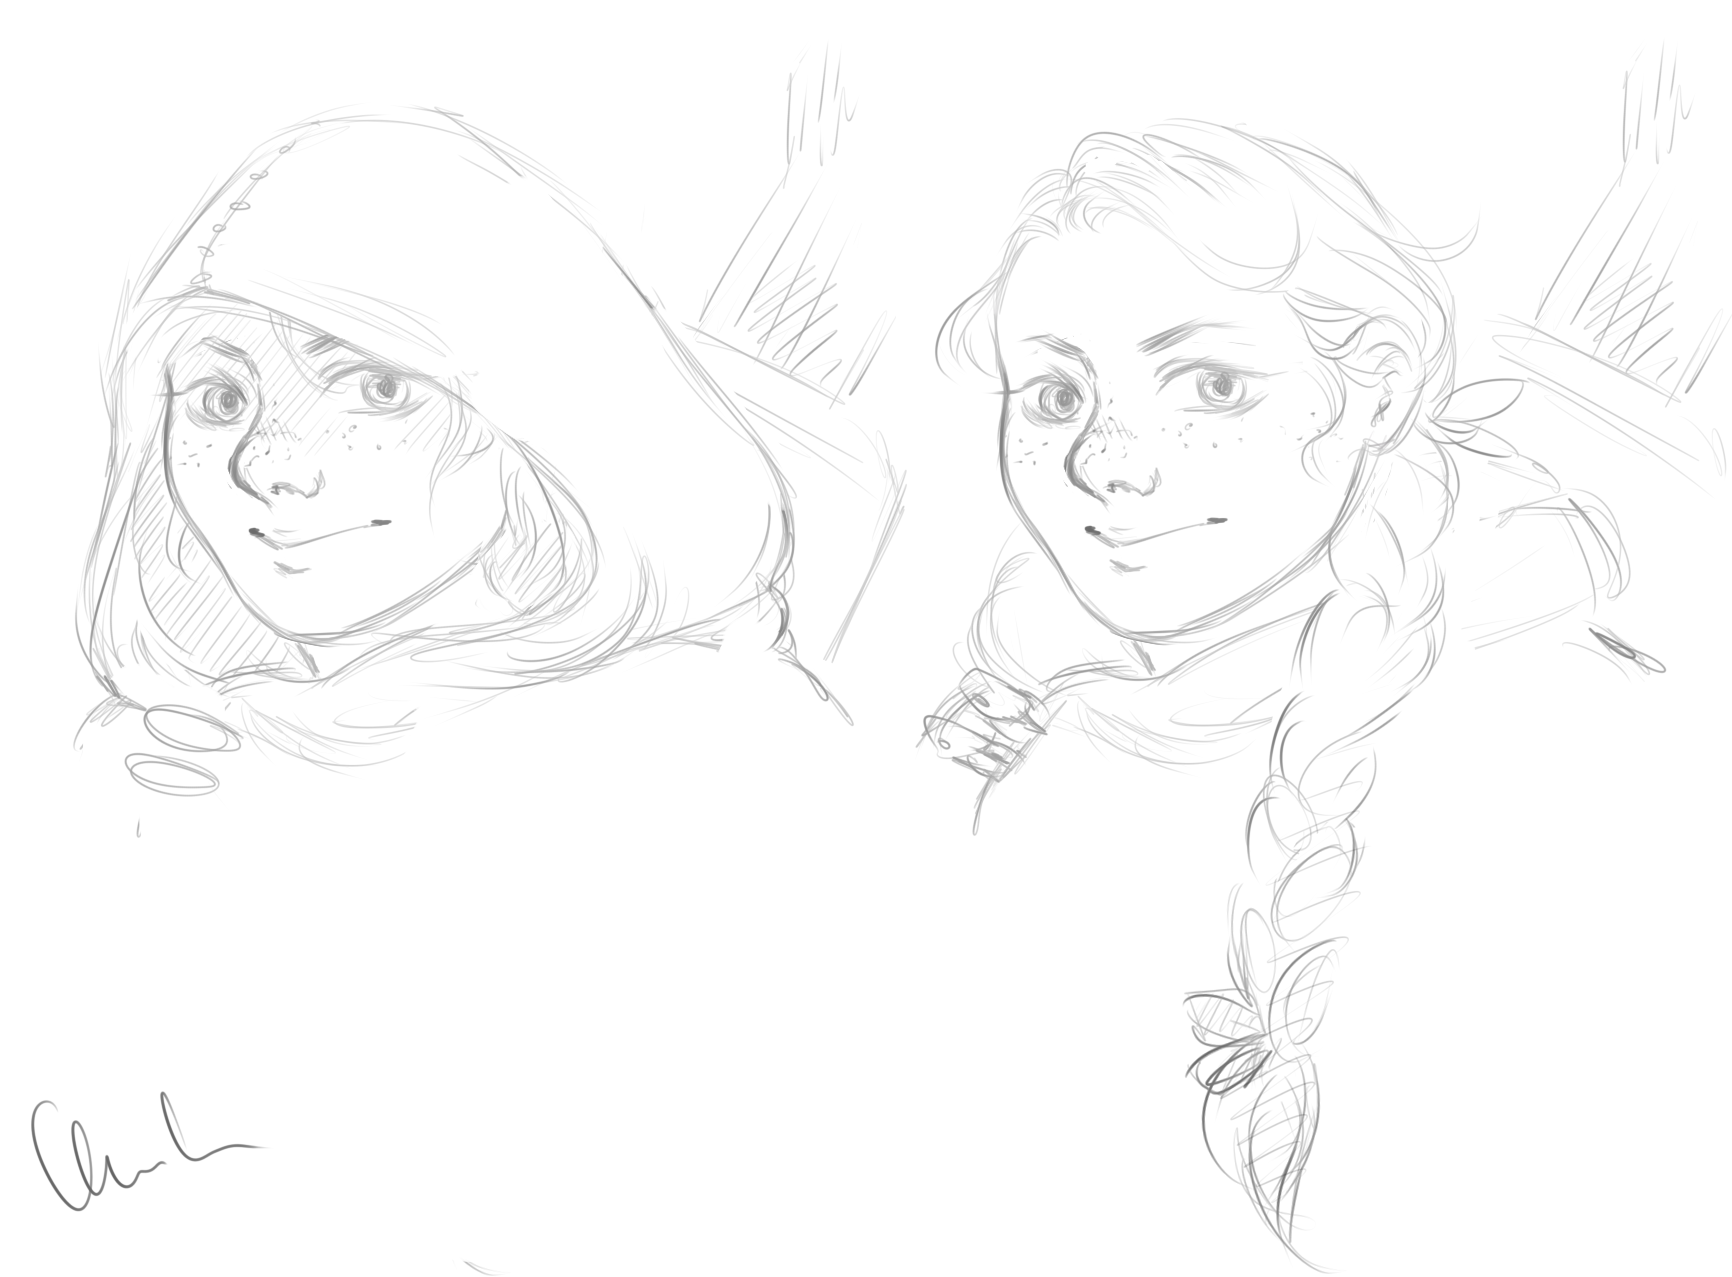
\includegraphics[width=0.9\textwidth]{Abbildungen/Abenteuer/Hauptcharaktere/spionin}
	\caption[Konzeptart Spionin]{Konzeptart Spionin als 16-Jährige während dem Hauptteil der Demo.}
	\label{fig:mc-spionin}
\end{figure}
